\chapter{Aprendizaje en Entornos Complejos}
% RECORDATORIO: La extensión máxima de este capítulo es de aproximadamente 5 páginas. 
% Se debe ser claro, conciso y priorizar el análisis crítico sobre la paja teórica.

\section{Introducción}
% Breve descripción del problema del aprendizaje en entornos complejos frente a los bandidos.
% Motivación: ¿Por qué pasar de entornos estáticos a MDPs (Procesos de Decisión de Markov)?
% Objetivos del informe: Evaluar y comparar métodos tabulares (SimpleGrid) y aproximados (Flappy Bird).
% Organización del capítulo.

El problema del bandido de k-brazos trata principalmente sobre el dilema de explotación-exploración en un contexto estático y estacionario: el agente selecciona acciones cuyas recompensas dependen únicamente de la acción elegida, sin que el entorno cambie como consecuencia de ella. No obstante, la toma de decisiones real rara vez carece de contexto o consecuencias. En entornos complejos, las acciones de un agente no solo determinan la recompensa inmediata, sino que también provocan una transición hacia un nuevo estado del entorno. La recompensa ya no depende solo de la acción, sino del par estado-acción, y las decisiones presentes condicionan las oportunidades futuras. Para modelar esta secuencialidad es necesario formular el problema como un \textbf{Proceso de Decisión de Markov} (MDP).

Bajo este marco, el agente debe aprender mediante la interacción y la experiencia directa, actualizando su política para maximizar la recompensa acumulada futura. A diferencia de los métodos de planificación clásica que requieren conocer explícitamente la dinámica del entorno, todos los algoritmos estudiados en este capítulo son \textbf{libres de modelo} (\textit{model-free}): el agente no tiene acceso previo a ese conocimiento y debe inferir su política únicamente a partir de las transiciones que observa al interactuar con el entorno.

Nuestro objetivo con este capítulo es evaluar el rendimiento, la estabilidad y la capacidad de convergencia de diversas técnicas de aprendizaje por refuerzo \textit{model-free} en dos entornos diferenciados por la dimensión de sus estados. En primer lugar, analizaremos empíricamente \textbf{métodos tabulares} clásicos (Monte Carlo y Diferencias Temporales) aplicados a un entorno de control discreto (SimpleGrid), donde el espacio de estados es finito y manejable. Posteriormente, dado que en problemas continuos la cantidad de estados hace inviable la representación tabular, estudiaremos la integración de \textbf{aproximadores de funciones} (SARSA semi-gradiente y Deep Q-Learning) aplicados a un entorno complejo y continuo como es Flappy Bird.

El resto del capítulo se organiza de la siguiente manera: la sección 2 formaliza el contexto teórico y los enfoques utilizados; la sección 3 detalla los algoritmos implementados; la sección 4 presenta el diseño experimental, los resultados empíricos y el análisis crítico de los métodos tabulares; y la sección 5 hace lo propio con los métodos aproximados.


\section{Desarrollo}
% Definición formal del problema: Estados, Acciones, Transiciones y Recompensas (MDP).
% Enfoques existentes: Diferencia conceptual entre Monte Carlo (episódico) y Diferencias Temporales (paso a paso).
% Contexto y antecedentes: La necesidad de aproximación de funciones cuando el espacio de estados crece (maldición de la dimensionalidad).
% Métodos utilizados: Breve justificación de por qué Sarsa/Q-Learning/MC para el grid y Semi-gradiente/DQN para Flappy Bird.

El aprendizaje por refuerzo en entornos complejos se formaliza habitualmente mediante un \textbf{Proceso de Decisión de Markov} (MDP). Un MDP se define por la tupla $\langle \mathcal{S}, \mathcal{A}, \mathcal{P}, \mathcal{R}, \gamma \rangle$, donde $\mathcal{S}$ es el conjunto de estados posibles, $\mathcal{A}$ es el conjunto de acciones, $\mathcal{P}(s'|s,a)$ representa la probabilidad de transición al estado $s'$ tras ejecutar la acción $a$ en el estado $s$, $\mathcal{R}(s,a)$ es la función de recompensa esperada y $\gamma \in [0, 1]$ es el factor de descuento. En cada instante de tiempo $t$, el agente observa un estado $S_t \in \mathcal{S}$, selecciona una acción $A_t \in \mathcal{A}$ siguiendo una política $\pi(a|s)$, y el entorno responde con un nuevo estado $S_{t+1}$ y una recompensa $R_{t+1}$. El objetivo es encontrar una política óptima $\pi_*$ que maximice el retorno esperado $$G_t = \sum_{k=0}^{\infty} \gamma^k R_{t+k+1}$$

El factor de descuento $\gamma$ controla el horizonte temporal efectivo del agente: valores próximos a cero producen agentes cortoplacistas que priorizan la recompensa inmediata, mientras que valores próximos a uno hacen que el agente valore en mayor medida las consecuencias futuras.

\subsection{Métodos tabulares}

Para resolver el MDP cuando el espacio de estados y acciones es discreto y abarcable, se emplean métodos tabulares que estiman el valor exacto de la función de acción-valor $Q(s, a)$. En la literatura destacan dos enfoques principales:
\begin{itemize}
    \item \textbf{Montecarlo (MC):} Aprende a partir de la experiencia generada en episodios completos. Actualiza las estimaciones de valor promediando los retornos empíricos $G_t$ obtenidos al llegar a un estado terminal. 
    \item \textbf{Diferencias Temporales (TD):} Aprende paso a paso sin esperar al final del episodio, basando su actualización en las estimaciones actuales de los estados siguientes (\textit{bootstrapping}). Algoritmos como SARSA (\textit{on-policy}) y Q-Learning (\textit{off-policy}) pertenecen a esta familia.
\end{itemize}

Bajo condiciones estándar (visita repetida de todos los pares estado-acción y tasa de aprendizaje decreciente apropiada) ambos enfoques garantizan la convergencia a los valores exactos de $Q^*$, lo que los convierte en métodos teóricamente sólidos para espacios de estados finitos.

\subsection{Métodos continuos}

Cuando nos enfrentamos a problemas con espacios de estados continuos o de alta dimensionalidad, la representación tabular se vuelve inviable debido a limitaciones drásticas de memoria y a la incapacidad de generalizar la experiencia a estados no visitados de forma eficiente. Para superar esto se recurre a la \textbf{aproximación de funciones}. En lugar de una tabla, se utiliza una función parametrizada con pesos $\theta$, de modo que $Q(s, a; \theta) \approx q_*(s, a)$. La optimización de estos pesos se realiza típicamente mediante técnicas de descenso del gradiente.

Sin embargo, esta extensión introduce un reto fundamental: las garantías de convergencia no se cumplen. Cuando la función aproximadora no es lineal (como una red neuronal profunda), la combinación del \textit{bootstrapping}, la correlación temporal entre muestras consecutivas y la inestabilidad del objetivo puede producir divergencia. Esta es precisamente la motivación de estabilización que incorpora Deep Q-Learning: el \textit{replay buffer} rompe la correlación temporal de las muestras y la red objetivo fija el objetivo de aprendizaje durante un número determinado de pasos, evitando que la red persiga un blanco que ella misma está desplazando.

\subsection{Entornos}

Para abordar este trabajo hemos escogido dos entornos de diferente naturaleza. 

Como \textbf{entorno discreto} hemos optado por \texttt{SimpleGrid}. Este entorno recrea una cuadrícula bidimensional clásica en la que un agente debe desplazarse desde una casilla de inicio hasta una meta esquivando trampas u obstáculos. El agente recibe un estado discreto definido únicamente por sus coordenadas actuales en el tablero, siendo el conjunto de posibles estados finito y, por tanto, ideal para ser abordado mediante métodos tabulares. La \textbf{función de recompensa} típica del entorno otorga $+1.0$ al agente por alcanzar la casilla objetivo, $-1.0$ por caer en una trampa, y una leve penalización de $-0.01$ por cada paso dado, incentivando así al agente a encontrar siempre la ruta más rápida posible.

\begin{figure}[H]
    \centering
    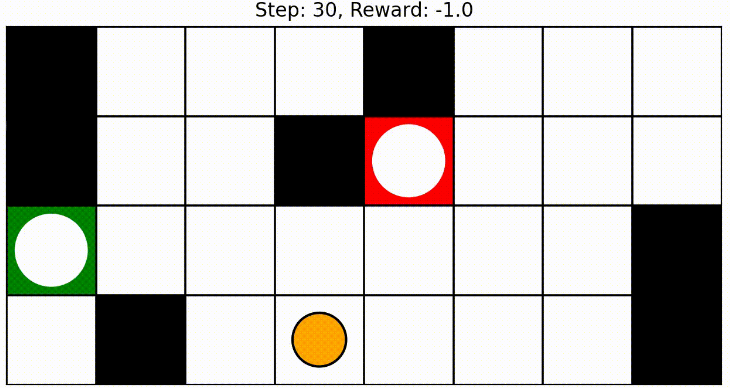
\includegraphics[width=0.7\linewidth]{images/entornos/simplegrid.png}
    \caption{Entorno Simplegrid}
    \label{fig:simplegrid}
\end{figure}

Nuestro segundo entorno, esta vez \textbf{continuo}, es \texttt{FlappyBird}. Este entorno recrea el famoso juego móvil Flappy Bird, en el que un pájaro avanza volando horizontalmente teniendo que aletear para sortear obstáculos en forma de tubería. El agente recibe un vector de estado continuo con 12 variables (altura, velocidad e inclinación del pájaro; posición de la tubería anterior y posterior...), siendo el conjunto de posibles estados continuo y, por tanto, inabarcable para un método de estados finitos. La \textbf{función de recompensa} propuesta por el repositorio del entorno otorga $+1.0$ al agente por atravesar un obstáculo, $+0.1$ por mantenerse vivo un frame, $-0.5$ por chocarse con el techo y $-1.0$ por morir.

\begin{figure}[H]
    \centering
    
\includegraphics[width=0.3\linewidth]{images/entornos/flappy_bird.png}
    \caption{Entorno Flappy Bird}
    \label{fig:flappybird}
\end{figure}


\section{Algoritmos}

En esta sección se describen brevemente los fundamentos de los algoritmos de aprendizaje por refuerzo empleados durante la fase experimental. 

\subsection{Monte Carlo}

\subsubsection{On-Policy}

El enfoque on-policy (basado en la política actual) evalúa y mejora de forma simultánea la misma política $\pi$ que el agente utiliza para tomar decisiones e interactuar con el entorno. Dado que los métodos de Monte Carlo no asumen ningún conocimiento previo de las dinámicas del sistema (son libres de modelo), es estrictamente necesario estimar la función de valor de acción $Q(s, a)$ en lugar de la función de valor de estado $V(s)$. Sin un modelo de transición, el agente necesita conocer el valor explícito de cada decisión posible para poder mejorar su política.

A diferencia de los métodos de diferencias temporales, Monte Carlo requiere que las tareas sean puramente episódicas. El algoritmo no actualiza su conocimiento paso a paso, sino que debe esperar a que el episodio finalice por completo (en el instante $T$) para observar el retorno total acumulado real, denotado como $G_t$, a partir de cada instante $t$:
$$G_t = R_{t+1} + \gamma R_{t+2} + \dots + \gamma^{T-1-t} R_T$$

Una vez que el episodio termina, el algoritmo promedia los retornos obtenidos para cada par estado-acción visitado. Si denotamos el número de veces que se ha visitado un par como $N(S_t, A_t)$, la actualización incremental se define como:
$$Q(S_t, A_t) \leftarrow Q(S_t, A_t) + \frac{1}{N(S_t, A_t)} \Big[ G_t - Q(S_t, A_t) \Big]$$
En entornos no estacionarios, el factor de promediado suele reemplazarse por una tasa de aprendizaje constante $\alpha$.

Un desafío crítico en el control on-policy es mantener el equilibrio entre la exploración de nuevas trayectorias y la explotación del conocimiento adquirido. Si la política se vuelve completamente codiciosa respecto a sus estimaciones iniciales, el agente podría no visitar nunca ciertas regiones del entorno, perdiéndose la oportunidad de descubrir estrategias superiores. Para evitar esto, habitualmente se emplea una política $\epsilon$-suave, siendo la estrategia $\epsilon$-greedy la más común. 

Esta técnica garantiza una exploración continua al asignar una pequeña probabilidad de selección a todas las acciones disponibles. Específicamente, la acción con el valor estimado más alto se selecciona con probabilidad $1 - \epsilon + \frac{\epsilon}{|\mathcal{A}(s)|}$, mientras que el resto de las acciones subóptimas se seleccionan de manera uniforme con una probabilidad de $\frac{\epsilon}{|\mathcal{A}(s)|}$. Esto asegura que el agente optimice las decisiones que ya han demostrado ser beneficiosas sin descartar la evaluación asintótica del resto de alternativas.

\subsubsection{Off-Policy}

El enfoque off-policy (fuera de política) ofrece una solución directa al dilema fundamental entre la exploración y la explotación al desacoplar completamente las políticas del agente. En este paradigma, el algoritmo utiliza dos estrategias distintas y simultáneas: la política objetivo ($\pi$), que es la que el agente intenta evaluar y optimizar hacia el ideal (generalmente una política determinista y puramente codiciosa), y la política de comportamiento ($b$), que es inherentemente exploratoria y es la que se utiliza realmente para interactuar con el entorno y generar los episodios.

Esta separación estructural permite aprender la estrategia óptima subyacente mientras el agente sigue explorando de forma ininterrumpida. Sin embargo, para que el aprendizaje cruzado sea teóricamente posible, debe cumplirse la suposición de cobertura: toda acción que la política objetivo $\pi$ pueda llegar a tomar, debe tener una probabilidad estrictamente mayor a cero de ser elegida por la política de comportamiento $b$ (es decir, $b(a|s) > 0$ siempre que $\pi(a|s) > 0$).

Dado que los retornos observados al final del episodio ($G_t$) se han generado siguiendo las probabilidades de la política $b$, promediarlos directamente para actualizar las estimaciones de $\pi$ introduciría un sesgo estadístico severo. Para corregir esta discrepancia de distribuciones, se aplica un mecanismo estadístico avanzado conocido como muestreo de importancia (\textit{importance sampling}). Este método pondera los retornos obtenidos según la probabilidad relativa de que la trayectoria observada bajo $b$ hubiera sido ejecutada exactamente igual bajo $\pi$.

El ratio de muestreo de importancia desde el instante temporal $t$ hasta el estado terminal en $T$ se define como el producto secuencial de estas probabilidades relativas:
\begin{equation}
\rho_{t:T-1} = \prod_{k=t}^{T-1} \frac{\pi(A_k \mid S_k)}{b(A_k \mid S_k)}
\end{equation}

Para actualizar la función de valor, el retorno real $G_t$ se escala multiplicándolo por este ratio $\rho_{t:T-1}$. Dependiendo del método de actualización, surgen dos variantes: el muestreo de importancia ordinario, que promedia de forma simple y suele sufrir de una varianza extrema e ilimitada (debido a que la multiplicación en cadena de probabilidades genera valores drásticamente altos o bajos), y el muestreo de importancia ponderado, que normaliza las actualizaciones reduciendo drásticamente la varianza a costa de introducir un pequeño sesgo inicial. En implementaciones prácticas, la variante ponderada resulta fundamental para asegurar la estabilidad y convergencia del algoritmo.

\subsection{SARSA}

SARSA constituye un método de aprendizaje por Diferencias Temporales (TD) enfocado en el control. Se clasifica estrictamente como un algoritmo \textit{on-policy}, lo que significa que evalúa y mejora de forma simultánea la política que el agente está ejecutando para interactuar con el entorno. A diferencia de los métodos \textit{off-policy}, SARSA aprende el valor exacto de la política de comportamiento, incorporando inherentemente los pasos de exploración (como las acciones aleatorias en una política $\epsilon$-greedy) dentro de sus estimaciones de valor.

Su nombre es un acrónimo que proviene de la secuencia exacta de eventos continuos que el algoritmo utiliza para realizar cada actualización: Estado actual ($S_t$), Acción actual elegida ($A_t$), Recompensa inmediata recibida ($R_{t+1}$), siguiente Estado observado ($S_{t+1}$) y, finalmente, la siguiente Acción elegida ($A_{t+1}$) de acuerdo a la política vigente. 

La regla de actualización matemática que rige el aprendizaje en SARSA se define formalmente como:
\begin{equation*}
Q(S_t, A_t) \leftarrow Q(S_t, A_t) + \alpha \Big[ R_{t+1} + \gamma Q(S_{t+1}, A_{t+1}) - Q(S_t, A_t) \Big]
\end{equation*}

En esta ecuación, $\alpha$ representa la tasa de aprendizaje y $\gamma$ el factor de descuento. El término $R_{t+1} + \gamma Q(S_{t+1}, A_{t+1})$ actúa como el objetivo hacia el cual se ajusta la estimación. Dado que este objetivo depende explícitamente de la acción $A_{t+1}$ que el agente efectivamente tomará, SARSA tiende a aprender políticas más conservadoras y seguras. Si explorar cerca de un estado de alto riesgo puede llevar a penalizaciones severas, SARSA ajustará los valores $Q$ a la baja para evitar esa región, reduciendo su propia tendencia a explorar.

A diferencia de los métodos de Monte Carlo, que requieren esperar estrictamente al final de un episodio para observar el retorno total acumulado ($G_t$) antes de aprender, SARSA aplica el principio de \textit{bootstrapping}. Esto significa que actualiza sus estimaciones paso a paso basándose parcialmente en otras estimaciones previas (el valor de $Q(S_{t}, A_{t})$). Esta característica fundamental permite que el aprendizaje ocurra de manera incremental y continua, resultando especialmente ventajoso en episodios extremadamente largos o en tareas continuas que carecen de un estado terminal.

\subsection{Q-Learning}

Q-Learning representa el algoritmo fundamental de aprendizaje por Diferencias Temporales (TD) enfocado en el control de tipo \textit{off-policy}. Introducido originalmente por Watkins en 1989 \cite{watkins1989learning}, este método supuso un avance crucial en el campo del Aprendizaje por Refuerzo, ya que busca aproximar directamente la función de valor de acción óptima, denotada como $Q^*$, independientemente de las acciones exploratorias que el agente esté realizando en ese momento bajo su política de comportamiento.

Para lograr este desacoplamiento entre la política objetivo que se optimiza y la política que interactúa con el entorno, Q-Learning incorpora el operador de maximización ($\max$) sobre las posibles acciones del estado siguiente ($S_{t+1}$) dentro de su regla de actualización:
\begin{equation*}
Q(S_t, A_t) \leftarrow Q(S_t, A_t) + \alpha \Big[ R_{t+1} + \gamma \max_{a} Q(S_{t+1}, a) - Q(S_t, A_t) \Big]
\end{equation*}

En esta expresión matemática, el objetivo queda definido por el término $R_{t+1} + \gamma \max_{a} Q(S_{t+1}, a)$. De esta forma, el algoritmo evalúa la transición actual asumiendo de manera optimista que en el futuro siempre se tomará la mejor decisión posible (la acción codiciosa que maximiza la estimación de $Q$). Esto ocurre de forma totalmente independiente a la acción real que el agente termine ejecutando en el siguiente paso, la cual podría ser aleatoria o subóptima si está bajo una estrategia de exploración como $\epsilon$-greedy.

Esta característica \textit{off-policy} contrasta fuertemente con algoritmos como SARSA. Mientras que SARSA aprende a alejarse de zonas de alto riesgo penalizando estados cercanos al peligro (porque reconoce que su propia exploración podría hacerle fallar), Q-Learning ignora los riesgos derivados de la exploración temporal y traza directamente la ruta ideal y más corta hacia la recompensa. 

Bajo las condiciones teóricas estándar de aproximación estocástica; es decir, asumiendo que todos los pares estado-acción continúan siendo visitados repetidamente y que la tasa de aprendizaje $\alpha$ decae de manera apropiada; esta actualización garantiza una convergencia estable hacia la estrategia óptima con probabilidad uno.

\subsection{SARSA Semi-Gradiente}
Para resolver problemas en entornos continuos, el espacio de estados es infinito (o gigantesco), por lo que es imposible almacenar los valores en una tabla clásica. En su lugar, se adapta SARSA, parametrizando la función de valor de acción $Q$ mediante un vector de pesos $\mathbf{w}$, denotada ahora como $\hat{q}(s, a, \mathbf{w})$. 

Al hacer esto, actualizar el conocimiento del agente ya no significa cambiar el valor de una celda en una tabla, sino ajustar los pesos $\mathbf{w}$ para modificar la forma de la función $Q$ en todo el entorno continuo. La ecuación de actualización es:

\begin{equation*}
\label{eq:sarsa_semigrad}
\begin{split}
\mathbf{w} \leftarrow \mathbf{w} + \alpha \Big[ & R_{t+1} + \gamma \hat{q}(S_{t+1}, A_{t+1}, \mathbf{w}) \\
& - \hat{q}(S_t, A_t, \mathbf{w}) \Big] \nabla_{\mathbf{w}} \hat{q}(S_t, A_t, \mathbf{w})
\end{split}
\end{equation*}

Desglosando la actualización de la función $Q$:

\begin{itemize}
    \item $\mathbf{w}$: Pesos que definen a la función $Q$ para el entorno continuo.
    \item $\hat{q}(S_t, A_t, \mathbf{w})$: Nuestra estimación actual de la función $Q$.
    \item En el corchete se mide la diferencia entre nuestra estimación y el objetivo temporal ($R_{t+1} + \gamma \hat{q}$).
    \item $\nabla_{\mathbf{w}} \hat{q}$: El gradiente de la función $Q$. Nos indica matemáticamente cómo mover los pesos $\mathbf{w}$ para corregir el error en nuestra estimación.
\end{itemize}

Al derivar la función para actualizar los pesos, notamos que el objetivo de nuestra actualización ($R_{t+1} + \gamma \hat{q}(S_{t+1}, A_{t+1}, \mathbf{w})$) también depende de los propios pesos $\mathbf{w}$. 

Se llama semi-gradiente porque hacemos una simplificación intencionada: ignoramos esta dependencia y tratamos al objetivo como una constante fija. Solo calculamos el gradiente de nuestra estimación actual.

\begin{algorithm}[H]
\caption{SARSA Semi-gradiente para entornos continuos}
\label{alg:sarsa_semigrad}
\begin{algorithmic}[1]
\Require $\alpha > 0$, $\gamma \in [0, 1]$, pesos iniciales $\mathbf{w}$
\For{cada episodio}
    \State Inicializar $S$ y elegir acción $A$ usando política sobre $\hat{q}$
    \While{$S$ no sea terminal}
        \State Ejecutar $A$, ver recompensa $R$ y nuevo estado $S'$
        \State Elegir siguiente acción $A'$ desde $S'$
        \If{$S'$ es terminal}
        \State $Obj \leftarrow R$
        \Else
        \State $Obj \leftarrow R + \gamma \hat{q}(S', A', \mathbf{w})$ 
        \EndIf
        \State $\mathbf{w} \leftarrow \mathbf{w} + \alpha \big[ Obj - \hat{q}(S, A, \mathbf{w}) \big] \nabla_{\mathbf{w}} \hat{q}(S, A, \mathbf{w})$
        \State $S \leftarrow S'$, $A \leftarrow A'$
    \EndWhile
\EndFor
\end{algorithmic}
\end{algorithm}

\subsection{Deep Q-Learning (DQN)}

Deep Q-Learning extiende los principios de Q-Learning para operar en entornos con espacios de estados continuos y de alta dimensionalidad, aproximando la función de acción-valor óptima mediante una red neuronal profunda parametrizada por $\theta$, de modo que $Q(s,a;\theta)\approx q^*(s,a)$. El objetivo de aprendizaje en cada paso es minimizar el error de diferencias temporales entre la estimación actual y el valor objetivo:
$$\mathcal{L}(\theta)=\mathbb{E}\left[\left(r + \gamma\max_{a'}Q(s',a';\theta^-)-Q(s,a;\theta\right)^2\right]$$
donde $\theta^-$ son los pesos de la red objetivo, distintos de $\theta$. La actualización de $\theta$ se realiza mendiante descenso del gradiente estocástico sobre esta pérdida.

El aprendizaje directo con redes neuronales sobre secuencias de experiencia correlacionadas temporalmente es inherentemente inestable. Para resolverlo, DQN incorpora dos mecanismos fundamentales.

\begin{itemize}
    \item \textbf{\textit{Replay buffer}}. Un \textit{buffer} \cite{mnih2015humanlevel} de capacidad fija almacena las transiciones $(s,a,r,s',\text{done})$ generadas durante la interacción con el entorno. En cada paso de entrenamiento, se extrae un lote aleatorio de transiciones del \textit{buffer} en lugar de utilizar la transición más reciente. Esto rompe la correlación temporal entre muestras consecutivas, convirtiendo el problema en uno más similar al aprendizaje supervisado estándar.

    \item \textbf{Target Network}. Una segunda red neuronal, parametrizada por $\theta^-$, se mantiene congenlada durante $N$ pasos y proporciona el valor objetivo $r + \gamma \max_{a'}Q(s',a';\theta^-)$. Sin este mecanismo, la red $Q_\theta$ perseguiría un objetivo que ella misma desplaza en cada actualización, creando un bucle de retroalimentación positiva que produce sobreestimación catastrófica de los valores Q. Cada $N$ pasos, los pesos de la red principal se copian a la objetivo.

    \item \textbf{Double Deep Q-Learning (DDQN)}. DQN estándar sufre de un sesgo de sobreestimación inherente al operador $\max$. Cuando los errores de estimación son independientes con media cero, la desigualdad de Jensen garantiza que $\mathbb{E}[\max_iX_i]\geq \max_i\mathbb{E}[X_i]$: el máximo de estimaciones ruidosas sobreestima sistemáticamente el máximo de los valores reales. Double DQN \cite{vanhasselt2016deep} mitiga este sesgo desacoplando la selección de la acción de su evaluación: la red principal $Q_\theta$ selecciona la acción más prometedora y la red objetivo $Q_{\theta^-}$ estima de forma independiente el valor $Q$ de esa acción. El objetivo es entonces:
    $$r + \gamma Q \left(s', \arg \max_{a'}Q(s',a';\theta);\theta^-\right)$$

\end{itemize}

\section{Métodos Tabulares}

\subsection{Entorno Simple Grid}

Para aumentar la complejidad y evaluar la capacidad de generalización, el entorno no utiliza un mapa fijo. En su lugar, se genera una cuadrícula procedural de 4x4 en cada episodio con una probabilidad del 25\% de aparición de obstáculos. Para evitar penalizar al agente en laberintos sin salida, se aplica un algoritmo de Búsqueda en Anchura (BFS) que garantiza que el mapa generado siempre tenga solución.

\subsection{Configuración Experimental}

Se han evaluado cuatro algoritmos: SARSA, Q-Learning, Monte Carlo On-Policy y Monte Carlo Off-Policy. Todos ellos se entrenan durante 1500 episodios, compartiendo hiperparámetros base como el factor de descuento ($\gamma=0.99$) y una tasa de exploración constante ($\epsilon=0.1$). Para los métodos de diferencias temporales, se utiliza una tasa de aprendizaje $\alpha=0.1$. Además, se impone un límite de 100 pasos por episodio para evitar bucles infinitos durante la fase de exploración.

\subsection{Métricas de Desempeño y Resultados}

El rendimiento de los modelos se ha medido utilizando tres métricas principales: la recompensa total acumulada, la longitud del episodio (número de pasos hasta la meta) y la tasa de éxito. Para visualizar claramente la tendencia de aprendizaje subyacente y reducir el ruido natural de la exploración, los datos de las gráficas se han suavizado mediante una media móvil de los últimos 50 episodios.

La siguiente figura agrupa la evolución temporal del rendimiento de los distintos métodos, permitiendo identificar rápidamente cuáles logran descifrar el entorno dinámico.

\begin{figure}[H]
    \centering
    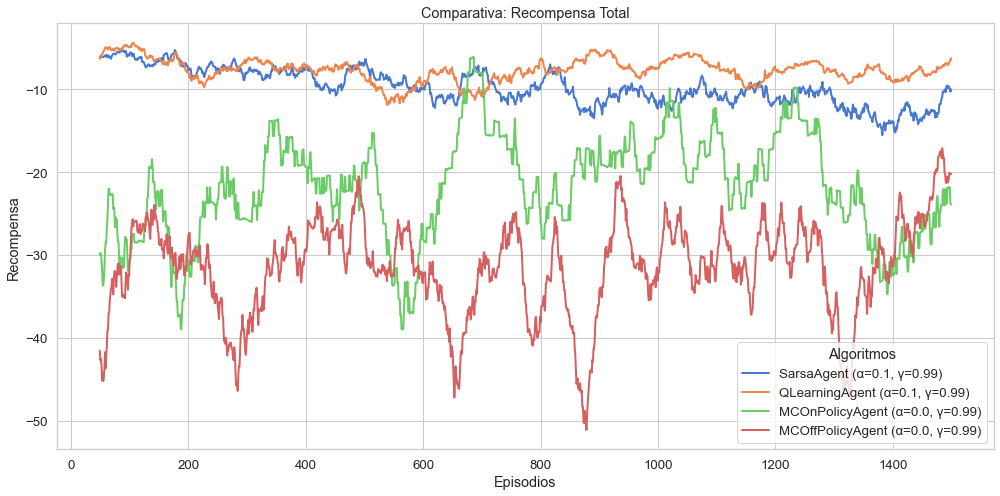
\includegraphics[width=\linewidth]{images/tabular/tabular.png}
    \caption{Comparativa del rendimiento global de los métodos tabulares en mapas generados proceduralmente.}
    \label{fig:comparativa_tabulares}
\end{figure}

\begin{figure}[H]
    \centering
    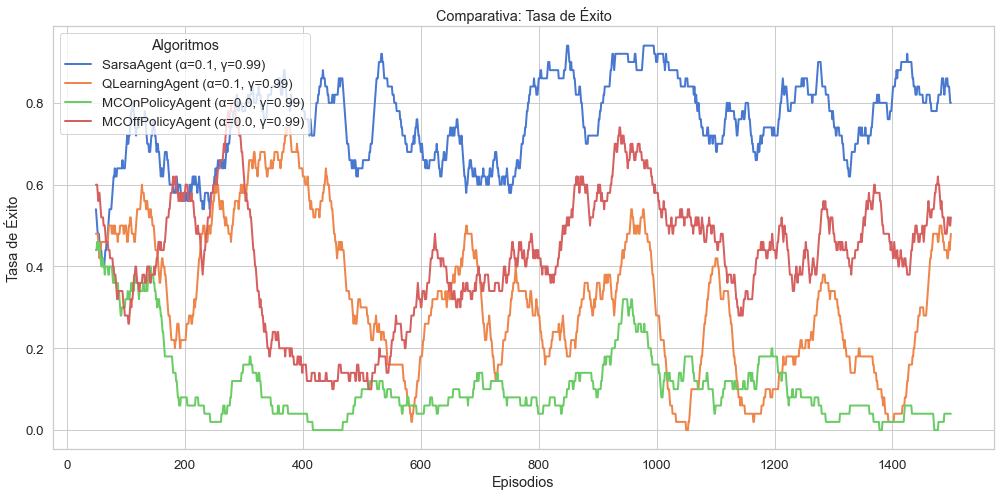
\includegraphics[width=\linewidth]{images/tabular/tasaExito.png}
    \caption{Comparativa de la tasa de éxito de los métodos tabulares en mapas generados proceduralmente.}
    \label{fig:exito_tabulares}
\end{figure}

Al analizar conjuntamente la evolución de la recompensa y la tasa de éxito (Figuras \ref{fig:comparativa_tabulares} y \ref{fig:exito_tabulares}), se observa una clara diferencia en el comportamiento de los algoritmos evaluados.

En la familia de diferencias temporales, \textbf{Q-Learning} (línea naranja) obtiene la mayor recompensa media, manteniéndose relativamente estable y cercano a los valores menos negativos durante gran parte del entrenamiento. Sin embargo, su tasa de éxito es altamente inestable, mostrando oscilaciones pronunciadas y periodos en los que el rendimiento cae significativamente.

Por otro lado, \textbf{SARSA} (línea azul) presenta una recompensa ligeramente inferior, pero mantiene una tasa de éxito mucho más alta y estable, situándose frecuentemente entre 0.7 y 0.9. Esto indica que, aunque su recompensa no sea la mejor, logra resolver el entorno con mayor consistencia.

En cuanto a los métodos de \textbf{Monte Carlo}, los resultados muestran un rendimiento claramente inferior. La variante \textbf{MC On-Policy} (línea verde) mantiene tanto la recompensa como la tasa de éxito en niveles muy bajos durante todo el entrenamiento, lo que indica una incapacidad para aprender una política eficaz en el entorno.

Finalmente, \textbf{MC Off-Policy} (línea roja) muestra cierto aprendizaje a lo largo del entrenamiento, alcanzando tasas de éxito moderadas en algunos periodos. No obstante, su recompensa acumulada sigue siendo la peor de todos los algoritmos y presenta una elevada variabilidad, lo que evidencia una política poco eficiente.

\subsection{Análisis}

La comparación entre las dos familias de algoritmos pone de manifiesto la importancia de la actualización incremental en entornos dinámicos.

Los métodos de \textbf{Monte Carlo} (MC) resultan menos adecuados para este tipo de problema. La variante \textbf{MC On-Policy} apenas consigue aprender una estrategia útil, manteniéndose durante todo el entrenamiento con tasas de éxito cercanas a cero. Por su parte, \textbf{MC Off-Policy} logra mejorar parcialmente su rendimiento, pero presenta una elevada varianza y una recompensa acumulada muy baja. Esto sugiere que esperar al final de cada episodio para actualizar los valores introduce demasiado retraso en la señal de aprendizaje.

En contraste, los métodos de diferencias temporales (TD) muestran un comportamiento mucho más efectivo. \textbf{Q-Learning} consigue maximizar mejor la recompensa esperada, pero su política es inestable y su tasa de éxito fluctúa considerablemente a lo largo del entrenamiento.

Por el contrario, \textbf{SARSA} demuestra ser el algoritmo más estable y consistente, manteniendo tasas de éxito elevadas durante la mayor parte del proceso de aprendizaje. Al actualizar sus valores siguiendo la política que realmente está ejecutando, tiende a adoptar un comportamiento más prudente y robusto frente a la variabilidad del entorno.

\section{Métodos Aproximados}

\subsection{Entorno Flappy Bird}

Sobre la función de recompensa base, introducimos un \textit{wrapper} de \textit{reward shaping} que añade una bonificación $r_{\alpha,t}\in(0,\alpha)$ proporcional a la proximidad vertical del pájaro al centro del hueco de la tubería siguiente:
$$q_t= q_{t,\text{base}} + r_{\alpha,t}$$
La intuición de esta heurística es que un pájaro que se mantiene alineado con el hueco necesitará menos correcciones bruscas para atravesarlo, lo que debería acelerar la convergencia.

\subsection{Configuración Experimental}

\subsubsection{SARSA Semi-Gradiente}

Se han definido dos estrategias diferentes construidas a partir de una misma base. Inicialmente, se podría plantear aproximar función $Q$ como tensor $n$-dimensional en el consultar valores según una discretización específica de las variables del entorno. Esta aproximación resulta inviable ya que puede dar lugar a tensores enormes si se divide el espacio continuo en muchas zonas discretas; o a imprecisión si no se realizan las suficientes divisiones necesarias para representar correctamente un espacio continuo. Por ello, decidimos utilizar un pequeño MLP de 2 capas ocultas de 64 neuronas que aprende a lo largo del tiempo a aproximar la función $Q$.

A partir de esta base, definimos el agente básico de SARSA semi-gradiente al que entrenamos para superar obstáculos. Cómo método adicional, decidimos añadir un sesgo off-policy mediante un buffer de repetición \cite{mnih2015humanlevel}, en el que se almacenarán las diferentes transiciones que van ocurriendo, de esta forma, podemos entrenar a la red de aproximación de $Q$ utilizado muestras aleatorias de dicho buffer, limitando la correlación temporal de las muestras utilizadas.

Las dos variantes del agente de SARSA semi-gradiente han sido entrenadas en 10000 episodios de simulación, estableciendo un umbral de de exploración bajo decrementado linealmente con el progreso del entrenamiento ($\epsilon = [0.1, 0.05])$.

\subsubsection{Deep Q-Learning}

El diseño experimental evalúa seis variantes algorítmicas que aíslan de forma controlada tres componentes críticos: el uso de red objetivo, la aplicación de \textit{reward shaping} y el uso de Double DQN. La tabla siguiente resume las configuraciones:

\begin{table}[htbp]
\centering
\begin{scriptsize}
\begin{tabular}{c l c c c}
\hline
\textbf{ID} & \textbf{Estrategia} & \textbf{T. Network} & \textbf{DDQN} & $\boldsymbol{\alpha}$ \textbf{(shaping)} \\
\hline
A & Vanilla DQN          & No & No & 0.00 \\
B & DQN Estándar         & Sí & No & 0.00 \\
C & DQN + S. leve   & Sí & No & 0.05 \\
D & DQN + S. moderado & Sí & No & 0.25 \\
E & DQN + S. agresivo & Sí & No & 0.50 \\
F & Double DQN           & Sí & Sí & 0.00 \\
\hline
\end{tabular}
\end{scriptsize}
\caption{Configuraciones experimentales evaluadas en el estudio de Deep Q-Learning.}
\label{tab:dqn_configs}
\end{table}

La Estrategia A actúa como línea base pura sin ningún mecanismo de estabilización, permitiendo cuantificar empíricamente el impacto de la red objetivo. La Estrategia B es la línea base moderna. Las Estrategias C, D y E estudian el efecto del \textit{reward shaping} a distintas intensidades. La Estrategia F evalúa si el desacoplamiento selección-evaluación de Double DQN produce políticas más robustas.

Todos los hiperparámetros no relacionados con la variante se mantienen constantes entre estrategias:

\begin{table}[htbp]
\centering
\begin{scriptsize}
\begin{tabular}{l c}
\hline
\textbf{Hiperparámetro} & \textbf{Valor} \\
\hline
Episodios de entrenamiento        & 2\,000 \\
Semillas por estrategia           & 5 \\
Capacidad del replay buffer       & 10\,000 \\
Mínimo de experiencias antes de entrenar & 1\,000 \\
Tamaño del mini-lote              & 64 \\
Neuronas por capa oculta (2 capas) & 128 \\
Tasa de aprendizaje ($\alpha$)    & $10^{-3}$ \\
Factor de descuento ($\gamma$)    & 0{,}99 \\
$\epsilon$ inicial / mínimo / decaimiento & 1{,}0 / 0{,}01 / 0{,}996 \\
Frecuencia de actualización de la red objetivo & 500 pasos \\
Pasos máximos por episodio        & 2\,000 \\
\hline
\end{tabular}
\end{scriptsize}
\caption{Hiperparámetros compartidos por todas las estrategias DQN.}
\label{tab:dqn_hyperparams}
\end{table}

El proceso de evaluación consta de dos fases para cada semilla:

\begin{itemize}
    \item \textbf{Entrenamiento}. Cada agente se entrena durante $2000$ episodios registrando la recompensa acumulada, la longitud del episodio, la pérdida y los valores Q máximos. Durante el entrenamiento se aplica un mecanismo de \textit{checkpointing}: se guardan los pesos de la red cada vez que la puntuación real media (medida en tuberías superadas, sin incluir el bonus de shaping) supera el mejor valor registrado en una ventana deslizante de $30$ episodios. Esto garantiza que la política presentada sea la mejor encontrada durante el entrenamiento, evitando que fluctuaciones tardías degraden el resultado final.

    \item \textbf{Evaluación}. Inmediatamente tras el entrenamiento, se carga el mejor modelo guardado, se fija $\epsilon=0$ y el agente se evalúa durante $100$ episodios sobre el entorno sin shaping. Esto permite una comparación directa y justa  entre todas las estrategias, incluyendo las que utilizaron recompensas modificadas durante el entrenamiento, ya que todas se miden sobre la misma señal de recompensa nativa.
\end{itemize}

Dado que cada estrategia se ejecuta con 5 semillas y se evalúa en 100 episodios por semilla, se obtienen 500 puntuaciones por estrategia sobre las que se calcula la media, mediana, desviación típica y máximo.

Una vez concluido el estudio exploratorio, las dos estrategias con mejor rendimiento se reentrenan durante $5000$ episodios con las mismas 5 semillas y la misma metodología de evaluación. El objetivo es determinar si la ventaja estadística observada a $2000$ episodios se mantiene o invierte con entrenamiento prolongado, y en particular si Double DQN, al producir estimaciones Q más conservadoras, se beneficia proporcionalmente más del entrenamiento extendido que DQN estándar.


\subsection{Métricas de Desempeño y Resultados}

Para el análisis de resultados en métodos continuos, dado que estamos en un entorno de juego, se han utilizado como métricas principales la recompensa acumulada durante la partida y la cantidad total de frames que nuestro pájaro ha sobrevivido, relacionada esta última directamente con la cantidad de obstáculos que se han superado.

\subsubsection{SARSA Semi-Gradiente}

En SARSA Semi-Gradiente compararemos en los dos agentes propuestos las métricas expuestas anteriormente. Además, utilizando los resultados de entrenamiento, se han realizado simulaciones con $\epsilon = 0$ para probar el comportamiento de los agentes únicamente explotando el comportamiento aprendido.

Véase que el agente SARSA Semi-Gradiente puramente on-policy no logra aprender en ningún momento los patrones necesarios para poder esquivar obstáculos. En la figura~\ref{fig:sarsasg_on_policy} no se aprecia una tendencia de crecimiento clara ni en la gráfica de recompensa acumulada ni en la de frames sobrevividos.

\begin{figure*}
    \centering
    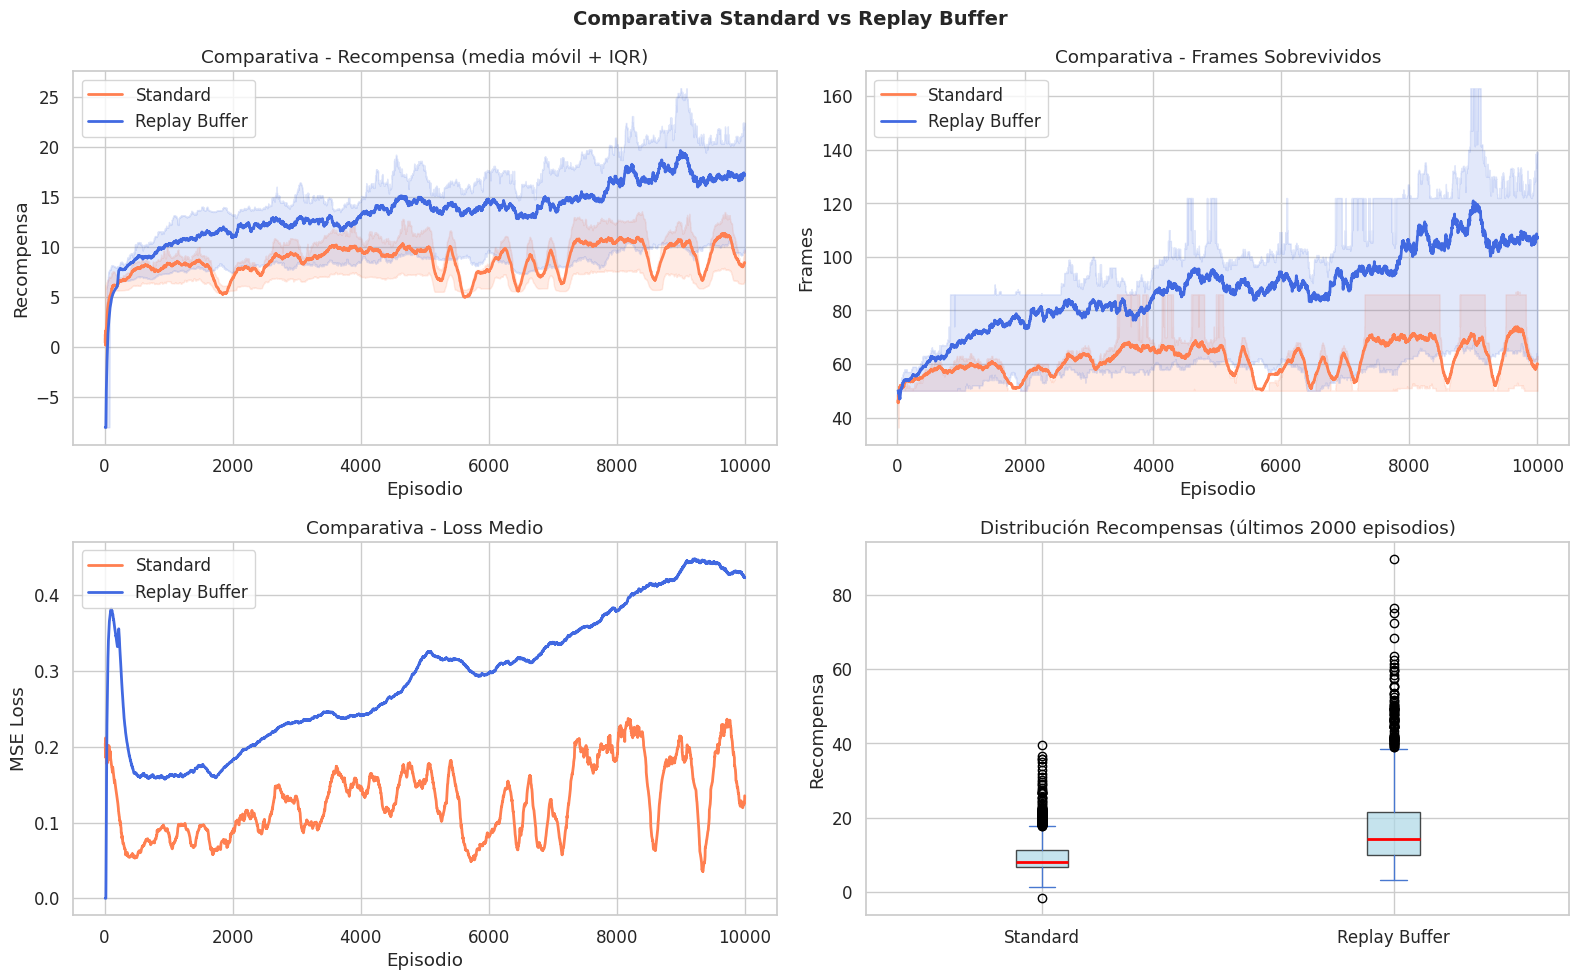
\includegraphics[width=\linewidth]{images/entornos/sarsasg.png}
    \caption{Métricas de entrenamiento SARSA Semi-Gradiente}
    \label{fig:sarsasg_on_policy}
\end{figure*}

Por el contrario, el agente con sesgo off-policy introducido mediante el buffer de repetición presenta varias características diferenciadoras que evidencian un mejor aprendizaje en la tarea de esquivar obstáculos. Lo más significativo es la estabilidad que presenta entre episodios; en comparación con su contra parte on-policy, este agente presenta mucha menos varianza en las diferentes métricas entre episodios. 

Se muestra perfectamente como conforme avanza el proceso de entrenamiento el crecimiento de recompensa acumulada y frames sobrevividos es lineal y estable. Nótese que incrementamos la penalización de pérdida con el paso de los episodios, penalizando al agente de forma proporcional al frame en el que falló su tarea. 

\begin{figure*}
    \centering
    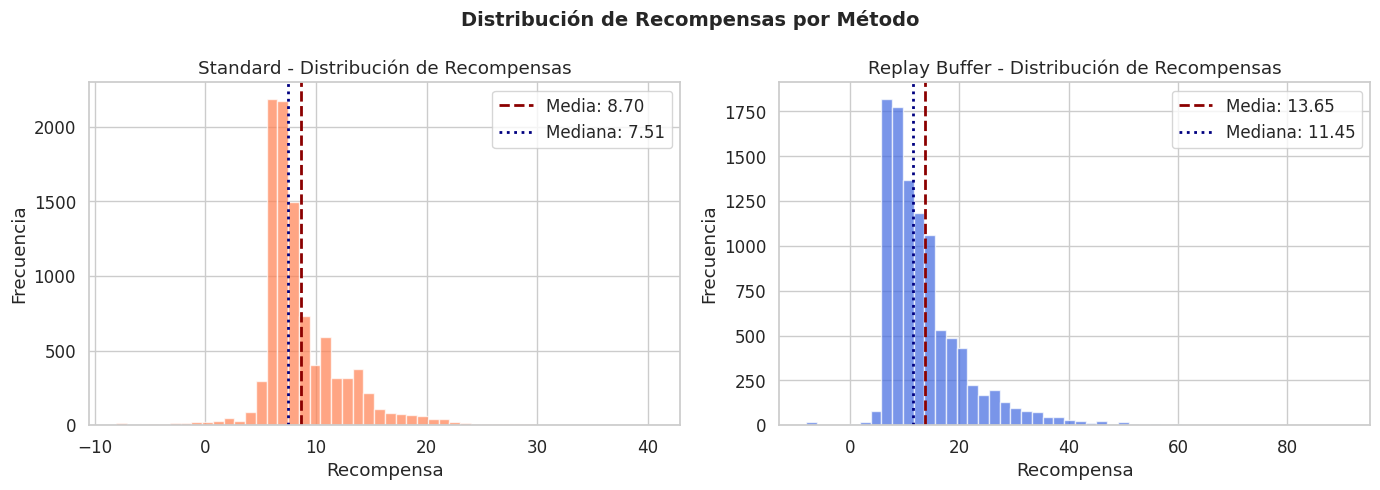
\includegraphics[width=0.9\linewidth]{images/entornos/recompensas.png}
    \caption{Distribución de recompensas durante el entrenamiento SARSA Semi-Gradiente}
    \label{fig:sarsasg_off_policy}
\end{figure*}

\begin{figure*}
    \centering
    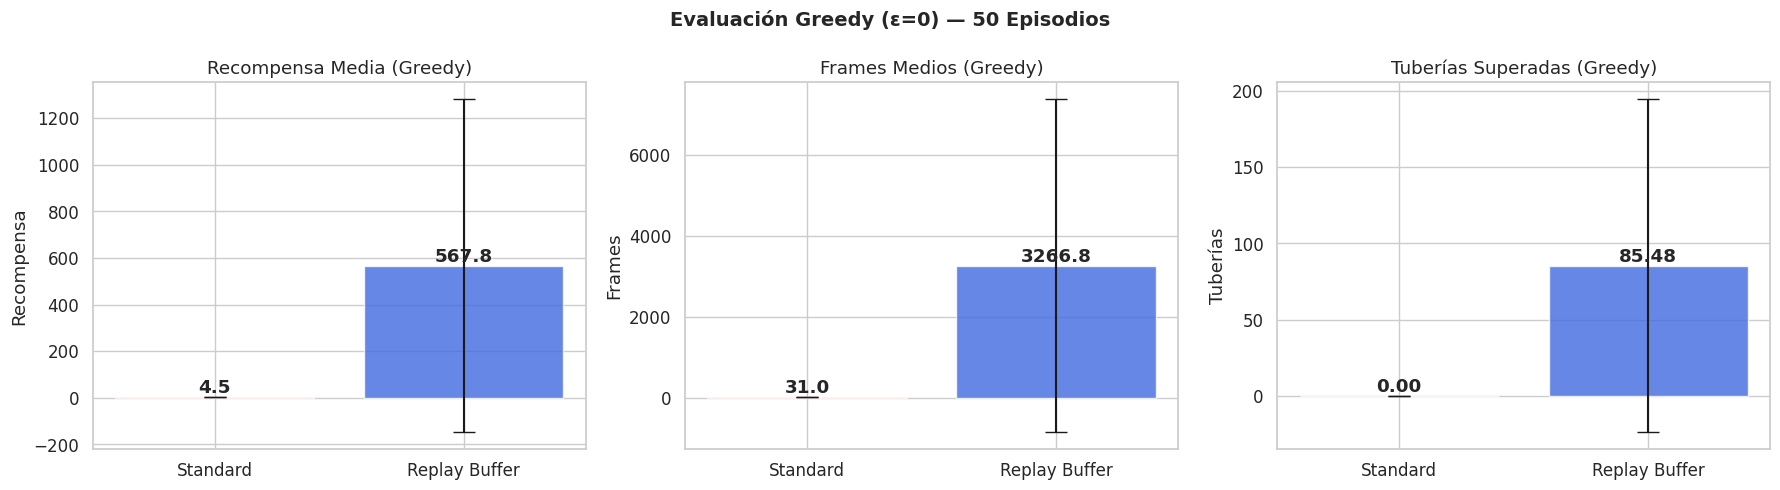
\includegraphics[width=\linewidth]{images/entornos/tuberias.png}
    \caption{Métricas de explotación SARSA Semi-Gradiente}
    \label{fig:sarsasg_off_policy}
\end{figure*}


La diferencia encontrada entre los agentes se debe a la forma en la que estamos entrenando a la red de aproximación de Q en el proceso de entrenamiento. La versión on-policy pura entrena a la red con las decisiones inmediatas que toma en el momento. Debido al pequeño tamaño del MLP y la cantidad de variables del entorno, se está introduciendo un sesgo de correlación temporal en la red, provocando que conforme avanza un episodio, el MLP olvide lo aprendido al inicio del mismo o en episodios de entrenamiento anteriores. Como solución se barajó incrementar el tamaño del MLP, pero eso podría no ser viable en ciertos entornos de despliegue realista, por lo que nos decantamos por el buffer de repetición.

La figura~\ref{fig:sarsasg_off_policy} muestra como, una vez entrenados, cuando aplicamos explotación pura, nuestra versión sesgada off-policy supera con creces a la versión de SARSA Semi-gradiente pura, ya que esta última no es capaz de cumplir su tarea en ningún episodio mientras que utilizando un buffer de repetición si es posible superar 85 tuberías de media por episodio, sobreviviendo más de 3000 frames.

Llegamos a la conclusión de que para tareas tan complejas como la que presenta nuestro entorno, utilizar métodos puramente on-policy es inviable, siendo necesaria información relativa a otras decisiones que se han tomado a lo largo del tiempo para facilitar tomar una decisión acertada en el presente.

\subsubsection*{Deep Q-Learning}

Para la comparación directa entre estrategias se utiliza exclusivamente la puntuación real obtenida en la fase de evaluación greedy (tuberías superadas en el entorno sin shaping), descartando las métricas de recompensa interna para las estrategias C, D y E, cuyas magnitudes no son comparables con las de A, B y F al incluir el bonus de shaping.

\textbf{Estudio exploratorio (2\,000 episodios).}
La siguiente tabla recoge el resumen estadístico del rendimiento real de las seis estrategias (500 evaluaciones por estrategia: 100 episodios $\times$ 5 semillas):
\begin{table}[h] % [b] pushes it to the bottom of the current column
\centering
% \resizebox shrinks the table to exactly the width of one column
\resizebox{\columnwidth}{!}{%
\begin{tabular}{l c c c c}
\hline
\textbf{Estrategia} & \textbf{Media} & \textbf{Mediana} & \textbf{Desv. típica} & \textbf{Máximo} \\
\hline
B - DQN Estándar         & 4{,}41 & 2{,}0 & 6{,}08 & 52 \\
F - Double DQN           & 3{,}54 & 2{,}0 & 4{,}75 & 37 \\
C - Shaping leve         & 2{,}72 & 1{,}0 & 3{,}61 & 34 \\
D - Shaping moderado     & 2{,}68 & 2{,}0 & 3{,}19 & 17 \\
A - Vanilla DQN          & 1{,}54 & 1{,}0 & 2{,}57 & 23 \\
E - Shaping agresivo     & 1{,}41 & 1{,}0 & 1{,}56 &  9 \\
\hline
\end{tabular}%
}
\caption{Rendimiento determinista final en el estudio exploratorio (100 episodios por semilla,
entorno sin shaping). Ordenado por media de tuberías superadas.}
\label{tab:dqn_exploratorio}
\end{table}

El ranking por media es: B $(4{,}41)$ $>$ F $(3{,}54)$ $>$ C $(2{,}72)$ $\approx$ D $(2{,}68)$ $\gg$ A $(1{,}54)$ $>$ E $(1{,}41)$.

\textbf{Análisis de cada componente experimental.}

\begin{itemize}

    \item \textit{Impacto de la Target Network (A vs.\ B).} La omisión de la red objetivo (Agente A) provoca una sobreestimación catastrófica de los valores Q, con picos superiores a 450 alrededor del episodio 300 (banda de confianza por encima de 700), seguidos de un colapso del aprendizaje. El mecanismo del fallo es el siguiente: sin red objetivo, la misma red $Q_\theta$ se usa tanto para seleccionar la mejor acción como para estimar su valor. Cuando $\theta$ se actualiza, el objetivo $r + \gamma \max_{a'} Q_\theta(s', a')$ cambia simultáneamente, creando un bucle de retroalimentación positiva. La red objetivo $Q_{\theta^-}$ rompe este ciclo fijando el objetivo durante $N$ pasos, estabilizando los valores Q por debajo de 15 en todas las estrategias restantes. El impacto sobre el rendimiento final es directo: A obtiene solo 1{,}54 tuberías de media frente a las 4{,}41 de B.

    \item \textit{Efecto del Reward Shaping (C, D, E).} Las tres variantes de shaping obtienen rendimientos inferiores a DQN estándar. El operador $\max_{a'} Q(s', a')$ produce un sesgo positivo inherente: cuando los errores de estimación tienen media cero, la desigualdad de Jensen garantiza que $\mathbb{E}[\max_i X_i] \geq \max_i \mathbb{E}[X_i]$. El shaping aditivo amplifica este efecto al inflar los retornos observados, empujando a la red a producir predicciones Q más altas. A mayor $\alpha$, mayor la distorsión. Además, el shaping empleado no es \textit{potential-based} en el sentido de Ng, Harada y Russell \cite{ng1999policy}, ya que no tiene la forma $F(s, a, s') = \gamma \Phi(s') - \Phi(s)$, y por tanto no preserva la política óptima. Con $\alpha = 0{,}50$ (Agente E), el bonus por frame ($+0{,}50$) domina la recompensa por tubo ($+1{,}00$), produciendo un agente que optimiza flotar centrado en lugar de cruzar tuberías (\textit{reward misalignment}), lo que explica su último puesto con solo 1{,}41 tuberías de media.

    \item \textit{Double DQN vs.\ DQN Estándar (F vs.\ B).} Para determinar si la diferencia entre B y F es estadísticamente significativa, aplicamos tests U de Mann-Whitney unilaterales sobre las 500 puntuaciones de cada estrategia. Esta prueba no paramétrica es adecuada dado que las distribuciones de puntuación en Flappy Bird no son normales. Los resultados se recogen en la siguiente tabla:
\end{itemize}

\begin{table}[htbp]
\centering
\begin{tabular}{l c c l}
\hline
\textbf{Hipótesis} & \textbf{Estadístico U} & \textbf{p-valor} & \textbf{Resultado} \\
\hline
$H_1$: F $>$ B & 118\,748{,}5 & 0{,}9195 & No significativo \\
$H_1$: F $>$ C & 142\,864{,}0 & $\approx 0$    & Significativo     \\
$H_1$: B $>$ C & 146\,430{,}5 & $\approx 0$    & Significativo     \\
\hline
\end{tabular}
\caption{Tests de Mann-Whitney U unilaterales ($\alpha = 0{,}05$) sobre las puntuaciones
de evaluación greedy del estudio exploratorio.}
\label{tab:mannwhitney}
\end{table}

B y F son estadísticamente indistinguibles a 2\,000 episodios ($p = 0{,}92$). El p-valor alto en la dirección F $>$ B sugiere incluso una tendencia contraria: B tiende a superar a F, aunque sin alcanzar significancia ($p_{\text{B}>\text{F}} \approx 0{,}08$). Ambas estrategias superan significativamente a C, D y E ($p \approx 0$). Dado este empate estadístico, se seleccionan B y F como finalistas para el estudio extendido.

\textbf{Estudio extendido (5\,000 episodios).}
Al prolongar el entrenamiento, el ranking se invierte:
\begin{table}[h]
\centering
% Shrinks the 7-column table to fit the column width
\resizebox{\columnwidth}{!}{
\begin{tabular}{l c c c c c c}
\hline
\textbf{Estrategia} & \textbf{Media} & \textbf{Mediana} & \textbf{Desv. típica} & \textbf{Máximo}
& \textbf{Media (2\,000 ep.)} & \textbf{Variación} \\
\hline
F --- Double DQN  & 4{,}97 & 2{,}0 & 7{,}24 & 52 & 3{,}54 & $+41\,\%$ \\
B --- DQN Estándar & 3{,}73 & 1{,}0 & 5{,}95 & 52 & 4{,}41 & $-15\,\%$ \\
\hline
\end{tabular}
}
\caption{Rendimiento determinista final en el estudio extendido (5\,000 episodios),
comparado con el exploratorio.}
\label{tab:dqn_extendido}
\end{table}

Double DQN mejora un 41\,\% respecto a su rendimiento exploratorio, mientras que DQN estándar retrocede un 15\,\%. Este resultado confirma la hipótesis teórica: al desacoplar la selección de la acción de su evaluación, Double DQN acumula menos sesgo de sobreestimación y se beneficia proporcionalmente más del entrenamiento prolongado. El retroceso de B sugiere que DQN estándar sufre de \textit{overfitting} temporal: encuentra buenas políticas en ventanas intermedias del entrenamiento, pero las pierde con episodios adicionales debido a la sobreestimación acumulativa que corrompe gradualmente la función Q. La figura~\ref{fig:dqn_loss_extendido} muestra la evolución de la pérdida en el estudio extendido para B y F, donde se aprecia la mayor estabilidad de F a lo largo de los 5\,000 episodios.

\subsubsection{Comparativa de métodos aproximados}

Experimentalmente, se ha observado que para este entorno en específico, nuestra versión de SARSA Semi-Gradiente sesgada ha funcionado mucho mejor que los métodos de Deep Q-Learning propuestos. Numéricamente, nuestra mejor versión de Deep Q-Learning supera una media de $4.41$ tuberías, mientras que SARSA-SG más de $85$.

Esto se puede justificar atendiendo a la naturaleza de ambos algoritmos. DQN es inherentemente optimista; sobre todo al principio del entrenamiento, la red comete errores, y algunas acciones no óptimas podrían tener valores altos asociados, lo que implica que el operador de maximización seleccionaría dichas acciones sobre otras que proporcionarían mejores resultados a largo plazo.

SARSA-SG es más precavido, y, con la introducción del sesgo del buffer de repetición, y al evaluar la política con exploración incluida, se rompe la correlación de los datos secuenciales y se obtiene una convergencia más suave hacia comportamientos que resuelven satisfactoriamente la tarea.

\clearpage

\begin{figure}
    \centering
    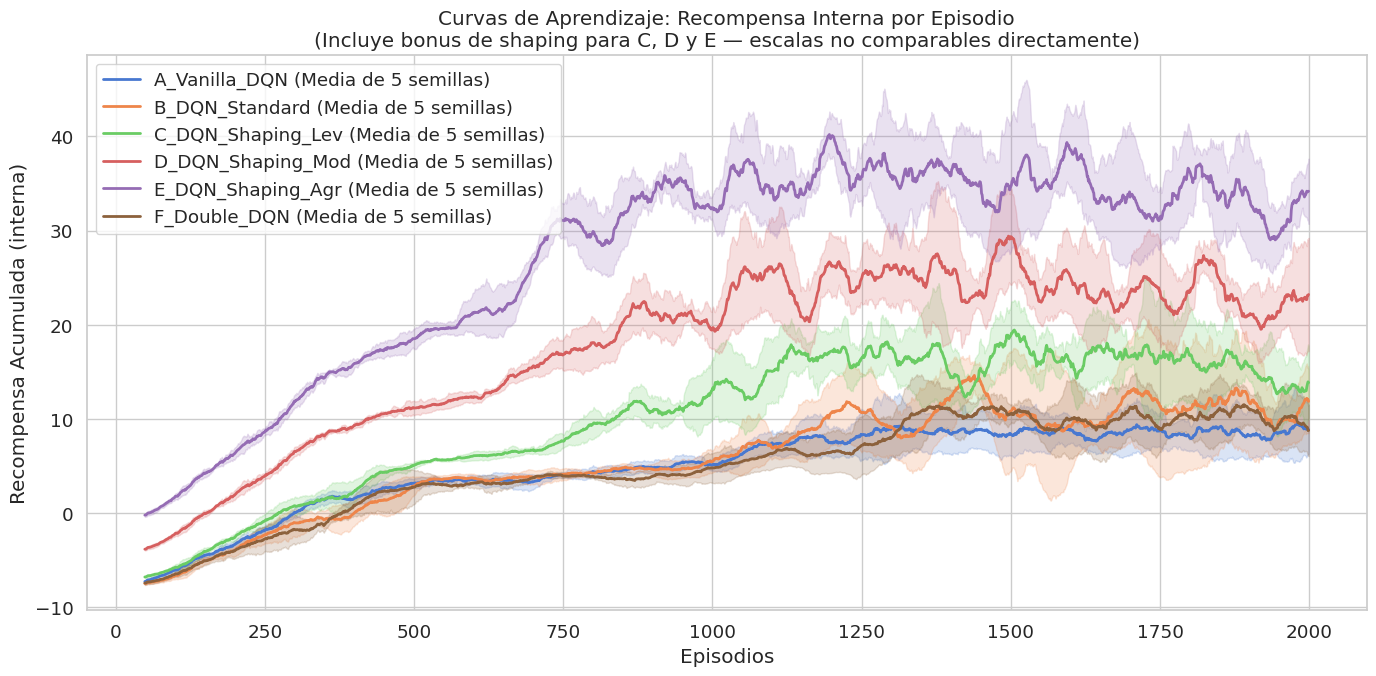
\includegraphics[width=\linewidth]{images/deepqlearning/dqn_img_00.png}
    \caption{Curvas de recompensa acumulada Deep Q-Learning}
    \label{fig:recompensa-dqn}
\end{figure}

\begin{figure}
    \centering
    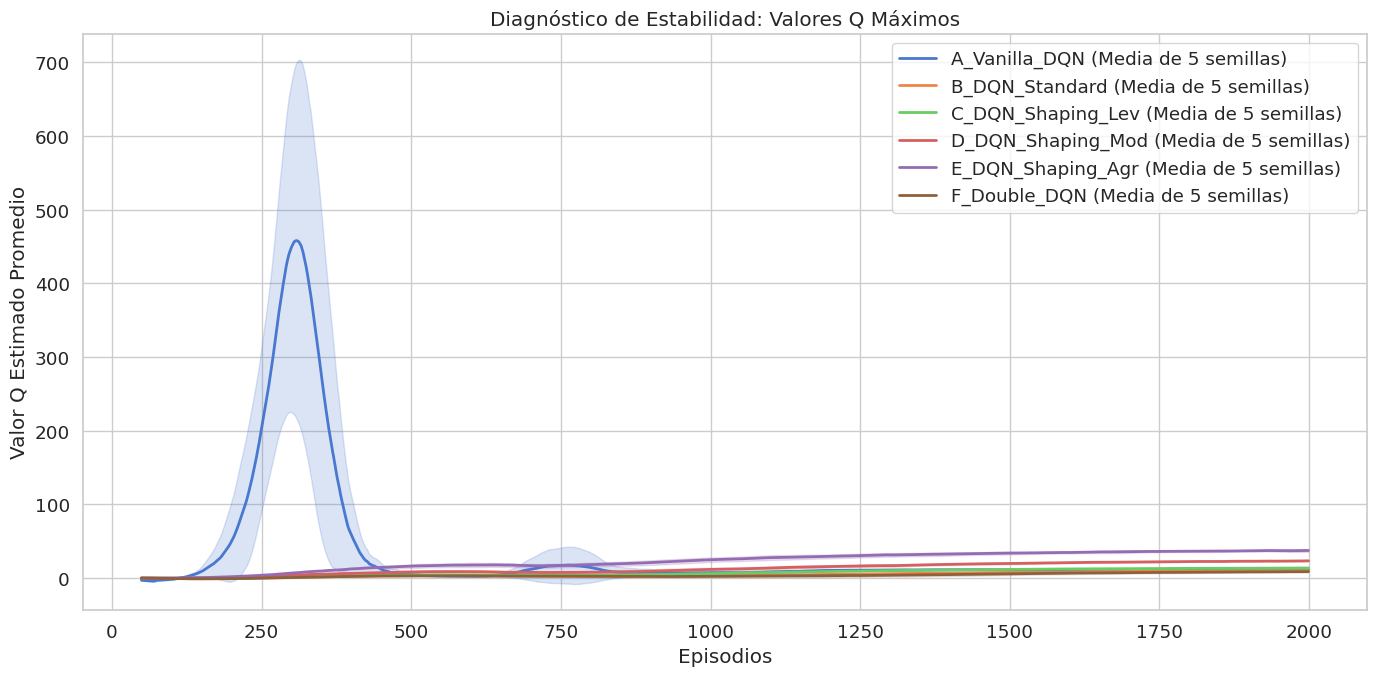
\includegraphics[width=\linewidth]{images/deepqlearning/dqn_img_01.png}
    \caption{Q valor predicho Deep Q-Learning}
    \label{fig:qvalor-dqn}
\end{figure}

\begin{figure}
    \centering
    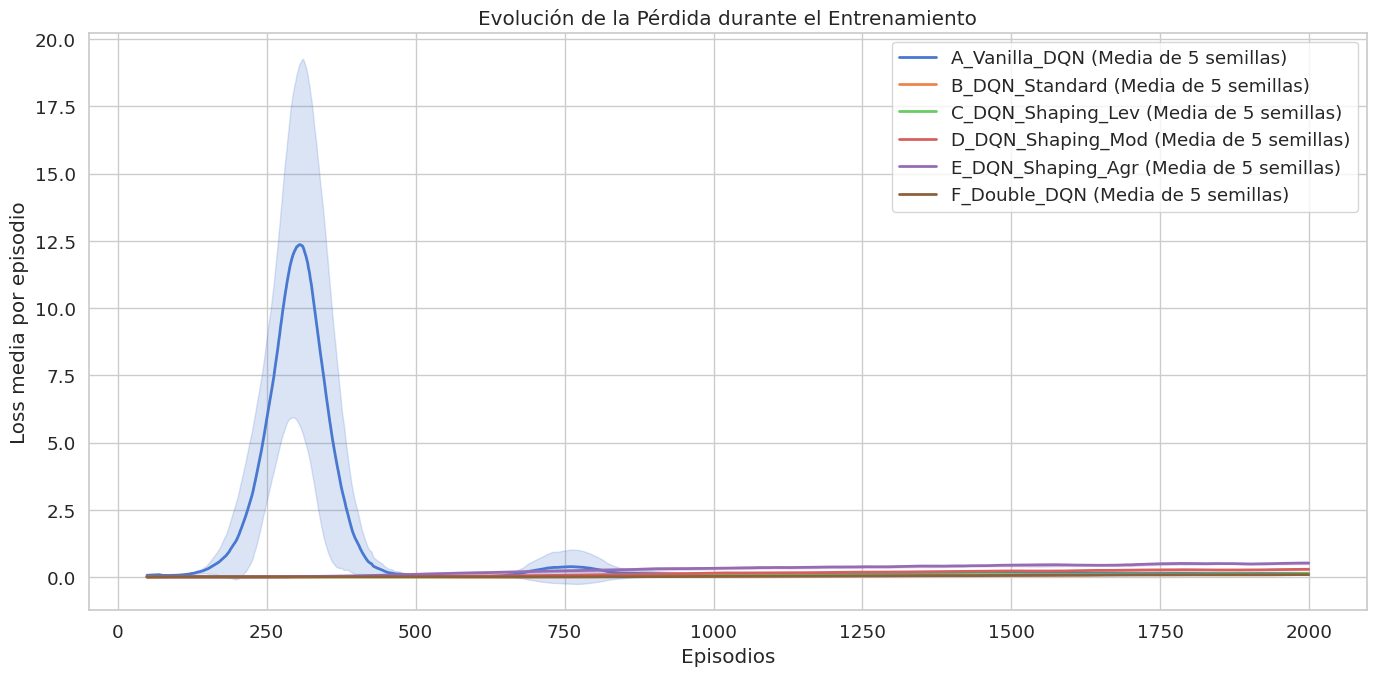
\includegraphics[width=\linewidth]{images/deepqlearning/dqn_img_02.png}
    \caption{Loss Deep Q-Learning}
    \label{fig:loss-dqn}
\end{figure}

\begin{figure}
    \centering
    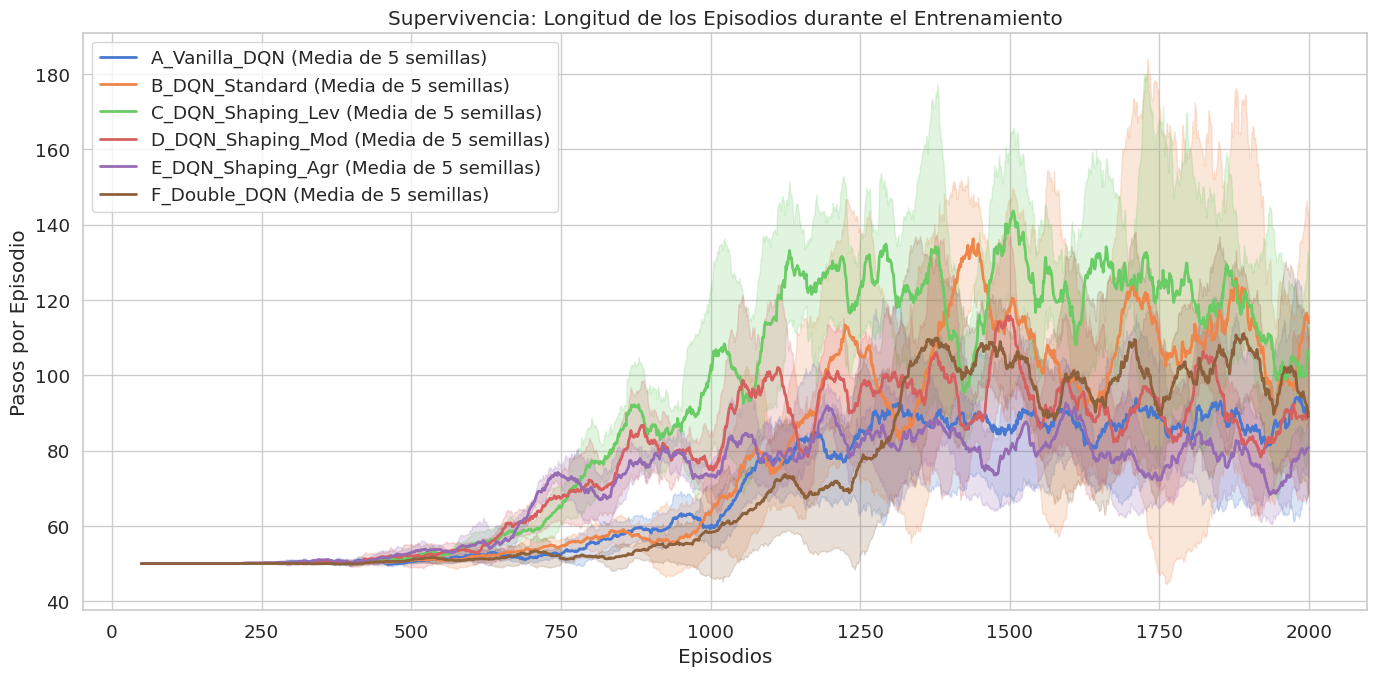
\includegraphics[width=\linewidth]{images/deepqlearning/dqn_img_03.png}
    \caption{Longitud de los episodios Deep Q-Learning}
    \label{fig:supervivencia-dqn}
\end{figure}

\begin{figure}
    \centering
    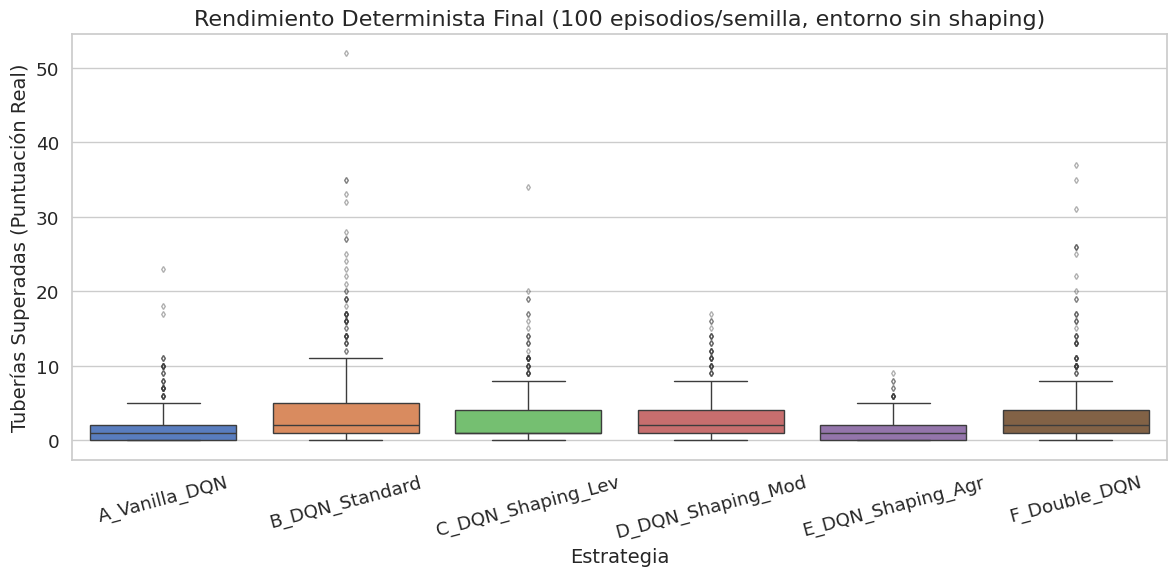
\includegraphics[width=\linewidth]{images/deepqlearning/dqn_img_04.png}
    \caption{Rendimiento de cada agente en Deep Q-Learning}
    \label{fig:rendimiento-dqn}
\end{figure}

\begin{figure}
    \centering
    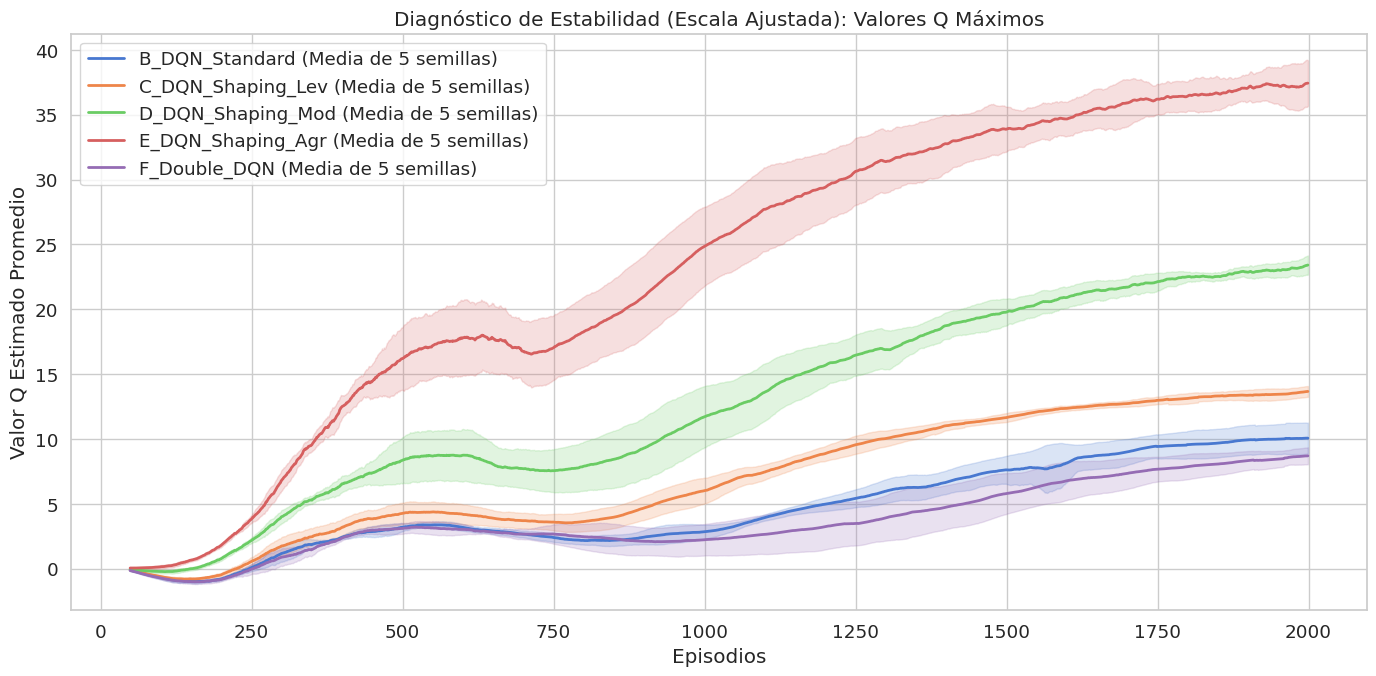
\includegraphics[width=\linewidth]{images/deepqlearning/dqn_img_05.png}
    \caption{Q valor predicho Deep Q-Learning (Sin estrategia A)}
    \label{fig:qvalorsina-dqn}
\end{figure}

\begin{figure}
    \centering
    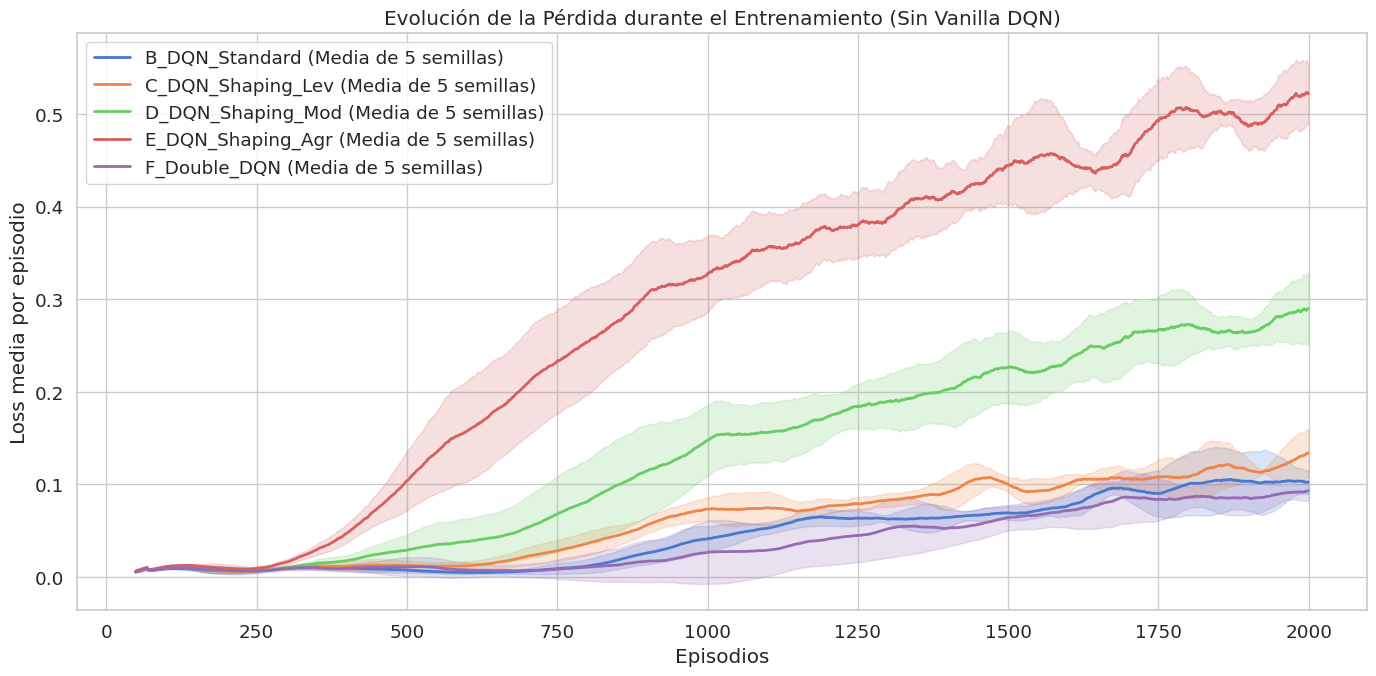
\includegraphics[width=\linewidth]{images/deepqlearning/dqn_img_06.png}
    \caption{Loss Deep Q-Learning (Sin estrategia A)}
    \label{fig:qvalorsina-dqn}
\end{figure}
